%%%%%%%%%%%%%%%%%%%%%%%%%%%%%%%%%%%%%%%%%%%%%%%%%%
\section{Results and interpretations}
%%%%%%%%%%%%%%%%%%%%%%%%%%%%%%%%%%%%%%%%%%%%%%%%%%

%-------------
The predicted number of SM background events and the number of events observed in data for each of the search regions defined in Section \ref{sec:trig} are summarized in Figure~\ref{fig:baseline_SR} and Table~\ref{tab:obs_vs_pred_37Bins}. 
%
Typically, the most significant background across the search regions comes from the SM \ttbar production or W-boson production, where either ${\rm W}\rightarrow \ell\nu$ and the lepton ($\ell={\rm e},\mu$) is not detected or ${\rm W}\rightarrow \tau\nu$ and the $\tau$ lepton decays hadronically. 
%
Generally, the next largest contribution comes from Z($\nu\nu$) production in association with jets (including heavy-flavour jets) in which the neutrino pair gives large \MET and the top quark conditions are satisfied by an accidental combination of the jets. 
%
The QCD multijet contribution and the conribution from other rare SM processes are subdominate across all bins. The largest rare SM process contribution (though still small) comes from \ttbarZ with the Z boson decaying into a pair of neutrinos. 

%%%%%%%%%%%%%%%%%%%%%%%%%%%%%%%%%%%%%%%%%%%%%%%%%%
\begin{figure}[htbp]
  \begin{center}
  \begin{tabular}{cc}
\hspace{-1.5cm}
  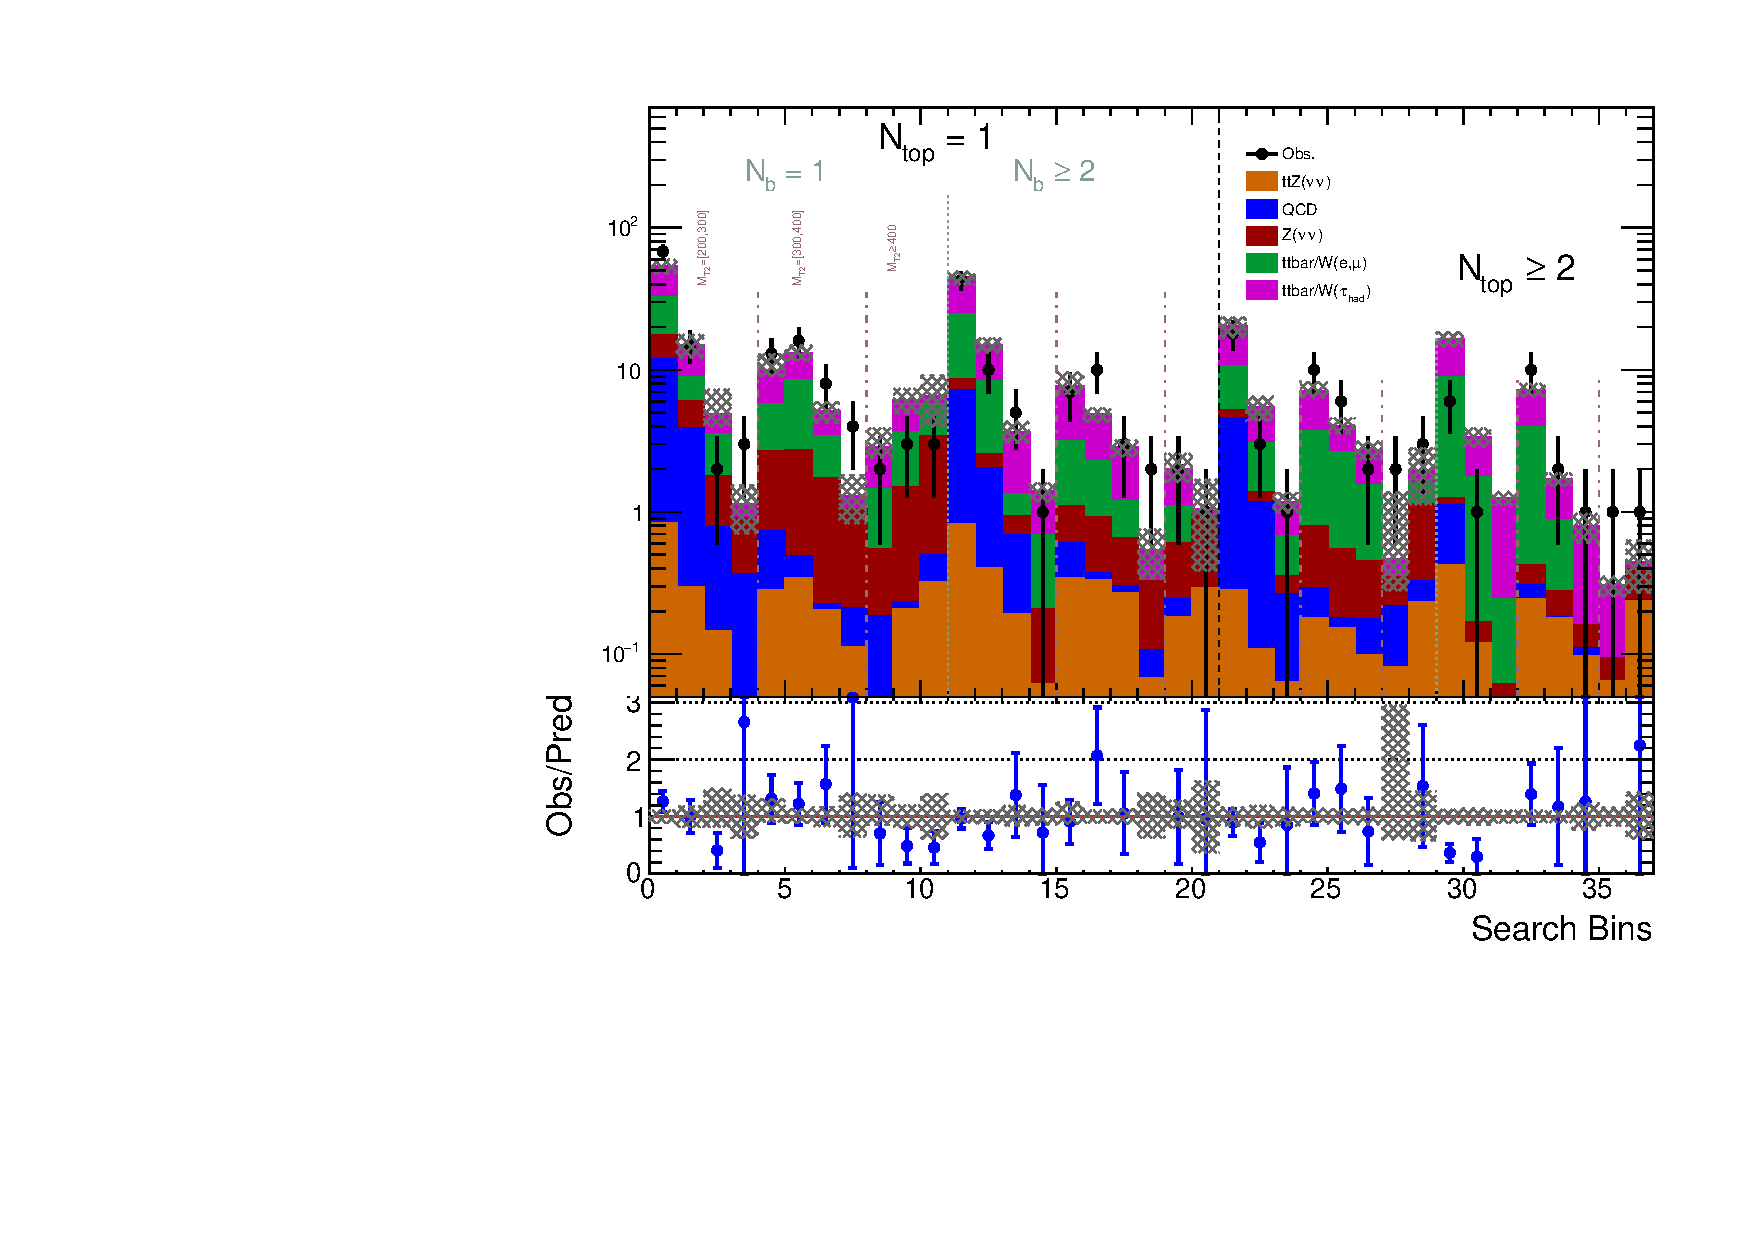
\includegraphics[angle=0,width=0.70\textwidth]{figures/UnblindPlots.pdf}
  \end{tabular}
  \caption{Data are shown as black points. The total predictions are shown in filled solid area. The bottom plot shows the ratio of data over total background prediction in each search bin. Only statistical uncertainties are propagated to the ratio.}
    \label{fig:baseline_SR}
  \end{center}
\end{figure}
%%%%%%%%%%%%%%%%%%%%%%%%%%%%%%%%%%%%%%%%%%%%%%%%%%

%%%%%%%%%%%%%%%%%%%%%%%%%%%%%%%%%%%%%%%%%%%%%%%%%%
\begin{landscape}
\newsavebox{\resBox}
\begin{table}[hp]
\centering
\caption{In the merged 37 bins: observed yields from the full luminosity of data compared to our total background predictions for the search bins.}
\label{tab:obs_vs_pred_37Bins}
\begin{lrbox}{\resBox}
%{\footnotesize
\begin{tabular}{|c|c|c|c|c||c|c||c|c|c|c|c|}
\hline
     SB &          \ntops &   \nbjets &   \MTTwo [\GeV] &     \MET [\GeV]  & Obs. & Sum. Pred. & Lost. Lep. & Had. Tau & Z($\nu\nu$)+Jets & QCD & ttZ \\
 \hline
              0 &               1 &               1 &         200-300 &         200-275  &     68 &  53.72 $^{+3.93}_{-3.78}$ $^{+6.44}_{-6.43}$ &  14.97 $^{+2.80}_{-2.63}$ $^{+2.23}_{-2.19}$ &  21.10 $^{+2.39}_{-2.32}$ $^{+1.39}_{-1.39}$ &   5.74 $^{+0.09}_{-0.09}$ $^{+1.56}_{-1.56}$ &  11.08 $^{+1.39}_{-1.39}$ $^{+5.66}_{-5.66}$ &   0.83 $^{+0.05}_{-0.05}$ $^{+0.29}_{-0.28}$ \\
 \hline
              1 &               1 &               1 &         200-300 &         275-350  &     15 &  14.95 $^{+2.18}_{-1.86}$ $^{+2.81}_{-2.81}$ &   2.84 $^{+1.57}_{-1.21}$ $^{+0.44}_{-0.44}$ &   6.15 $^{+1.29}_{-1.17}$ $^{+0.47}_{-0.47}$ &   2.11 $^{+0.05}_{-0.05}$ $^{+0.67}_{-0.67}$ &   3.56 $^{+0.80}_{-0.80}$ $^{+2.65}_{-2.65}$ &   0.30 $^{+0.03}_{-0.03}$ $^{+0.10}_{-0.10}$ \\
 \hline
              2 &               1 &               1 &         200-300 &         350-450  &      2 &   4.88 $^{+1.64}_{-1.16}$ $^{+2.44}_{-0.90}$ &   1.75 $^{+1.48}_{-1.07}$ $^{+0.30}_{-0.30}$ &   1.33 $^{+0.64}_{-0.33}$ $^{+0.18}_{-0.18}$ &   1.01 $^{+0.03}_{-0.03}$ $^{+0.53}_{-0.53}$ &   0.64 $^{+0.32}_{-0.32}$ $^{+2.35}_{-0.64}$ &   0.14 $^{+0.02}_{-0.02}$ $^{+0.05}_{-0.05}$ \\
 \hline
              3 &               1 &               1 &         200-300 &            450+  &      3 &   1.13 $^{+1.06}_{-0.23}$ $^{+0.43}_{-0.43}$ &   0.00 $^{+0.88}_{-0.00}$ $^{+0.00}_{-0.00}$ &   0.22 $^{+0.56}_{-0.09}$ $^{+0.03}_{-0.04}$ &   0.54 $^{+0.02}_{-0.02}$ $^{+0.29}_{-0.29}$ &   0.34 $^{+0.21}_{-0.21}$ $^{+0.31}_{-0.31}$ &   0.02 $^{+0.01}_{-0.01}$ $^{+0.01}_{-0.01}$ \\
 \hline
              4 &               1 &               1 &         300-400 &         200-275  &     13 &   9.90 $^{+1.84}_{-1.53}$ $^{+3.12}_{-0.97}$ &   3.02 $^{+1.47}_{-1.18}$ $^{+0.48}_{-0.47}$ &   4.18 $^{+1.11}_{-0.96}$ $^{+0.32}_{-0.32}$ &   1.96 $^{+0.05}_{-0.05}$ $^{+0.63}_{-0.63}$ &   0.45 $^{+0.09}_{-0.09}$ $^{+3.00}_{-0.45}$ &   0.28 $^{+0.03}_{-0.03}$ $^{+0.09}_{-0.09}$ \\
 \hline
              5 &               1 &               1 &         300-400 &         275-350  &     16 &  13.08 $^{+2.39}_{-2.09}$ $^{+1.78}_{-1.49}$ &   5.75 $^{+2.07}_{-1.80}$ $^{+0.92}_{-0.91}$ &   4.60 $^{+1.19}_{-1.06}$ $^{+0.75}_{-0.74}$ &   2.24 $^{+0.06}_{-0.06}$ $^{+0.89}_{-0.89}$ &   0.15 $^{+0.05}_{-0.05}$ $^{+0.97}_{-0.15}$ &   0.34 $^{+0.03}_{-0.03}$ $^{+0.12}_{-0.12}$ \\
 \hline
              6 &               1 &               1 &         300-400 &         350-450  &      8 &   5.09 $^{+1.70}_{-1.11}$ $^{+0.89}_{-0.88}$ &   1.65 $^{+1.51}_{-0.97}$ $^{+0.32}_{-0.32}$ &   1.71 $^{+0.77}_{-0.53}$ $^{+0.20}_{-0.20}$ &   1.51 $^{+0.04}_{-0.04}$ $^{+0.80}_{-0.80}$ &   0.02 $^{+0.05}_{-0.05}$ $^{+0.06}_{-0.02}$ &   0.20 $^{+0.03}_{-0.03}$ $^{+0.07}_{-0.07}$ \\
 \hline
              7 &               1 &               1 &         300-400 &            450+  &      4 &   1.30 $^{+1.08}_{-0.14}$ $^{+0.53}_{-0.47}$ &   0.00 $^{+0.91}_{-0.00}$ $^{+0.00}_{-0.00}$ &   0.25 $^{+0.56}_{-0.12}$ $^{+0.04}_{-0.04}$ &   0.84 $^{+0.03}_{-0.03}$ $^{+0.45}_{-0.45}$ &   0.10 $^{+0.07}_{-0.07}$ $^{+0.28}_{-0.10}$ &   0.11 $^{+0.02}_{-0.02}$ $^{+0.04}_{-0.04}$ \\
 \hline
              8 &               1 &               1 &            400+ &         200-350  &      2 &   2.83 $^{+1.28}_{-0.79}$ $^{+1.06}_{-0.43}$ &   0.91 $^{+0.99}_{-0.52}$ $^{+0.20}_{-0.19}$ &   1.38 $^{+0.81}_{-0.59}$ $^{+0.22}_{-0.22}$ &   0.36 $^{+0.02}_{-0.02}$ $^{+0.28}_{-0.28}$ &   0.15 $^{+0.05}_{-0.05}$ $^{+0.98}_{-0.15}$ &   0.04 $^{+0.01}_{-0.01}$ $^{+0.01}_{-0.01}$ \\
 \hline
              9 &               1 &               1 &            400+ &         350-450  &      3 &   6.16 $^{+2.12}_{-1.52}$ $^{+1.24}_{-1.24}$ &   2.15 $^{+1.85}_{-1.26}$ $^{+0.41}_{-0.40}$ &   2.51 $^{+1.02}_{-0.85}$ $^{+0.45}_{-0.45}$ &   1.26 $^{+0.04}_{-0.04}$ $^{+1.08}_{-1.08}$ &   0.02 $^{+0.05}_{-0.05}$ $^{+0.07}_{-0.02}$ &   0.21 $^{+0.03}_{-0.03}$ $^{+0.07}_{-0.07}$ \\
 \hline
             10 &               1 &               1 &            400+ &            450+  &      3 &   6.55 $^{+2.11}_{-1.45}$ $^{+2.64}_{-2.59}$ &   2.33 $^{+1.98}_{-1.37}$ $^{+0.48}_{-0.48}$ &   0.79 $^{+0.73}_{-0.47}$ $^{+0.12}_{-0.12}$ &   2.93 $^{+0.06}_{-0.06}$ $^{+2.53}_{-2.53}$ &   0.18 $^{+0.10}_{-0.10}$ $^{+0.52}_{-0.18}$ &   0.32 $^{+0.03}_{-0.03}$ $^{+0.11}_{-0.11}$ \\
 \hline
             11 &               1 &              2+ &         200-300 &         200-275  &     43 &  44.60 $^{+4.15}_{-4.00}$ $^{+4.82}_{-4.80}$ &  16.25 $^{+3.17}_{-3.02}$ $^{+2.48}_{-2.44}$ &  19.81 $^{+2.44}_{-2.38}$ $^{+1.33}_{-1.33}$ &   1.38 $^{+0.04}_{-0.04}$ $^{+0.96}_{-0.96}$ &   6.33 $^{+1.10}_{-1.10}$ $^{+3.78}_{-3.78}$ &   0.83 $^{+0.05}_{-0.05}$ $^{+0.27}_{-0.27}$ \\
 \hline
             12 &               1 &              2+ &         200-300 &         275-350  &     10 &  14.95 $^{+2.64}_{-2.35}$ $^{+1.80}_{-1.79}$ &   5.72 $^{+2.10}_{-1.80}$ $^{+0.89}_{-0.88}$ &   6.67 $^{+1.51}_{-1.40}$ $^{+0.49}_{-0.49}$ &   0.53 $^{+0.03}_{-0.03}$ $^{+0.39}_{-0.39}$ &   1.63 $^{+0.57}_{-0.57}$ $^{+1.43}_{-1.43}$ &   0.40 $^{+0.04}_{-0.04}$ $^{+0.14}_{-0.14}$ \\
 \hline
             13 &               1 &              2+ &         200-300 &         350-450  &      5 &   3.63 $^{+1.54}_{-0.89}$ $^{+0.71}_{-0.58}$ &   0.39 $^{+1.20}_{-0.39}$ $^{+0.07}_{-0.07}$ &   2.30 $^{+0.94}_{-0.76}$ $^{+0.21}_{-0.21}$ &   0.26 $^{+0.02}_{-0.02}$ $^{+0.21}_{-0.21}$ &   0.49 $^{+0.26}_{-0.26}$ $^{+0.64}_{-0.49}$ &   0.19 $^{+0.02}_{-0.02}$ $^{+0.07}_{-0.07}$ \\
 \hline
             14 &               1 &              2+ &         200-300 &            450+  &      1 &   1.39 $^{+1.48}_{-0.66}$ $^{+0.23}_{-0.21}$ &   0.48 $^{+1.30}_{-0.48}$ $^{+0.13}_{-0.13}$ &   0.71 $^{+0.71}_{-0.44}$ $^{+0.10}_{-0.10}$ &   0.14 $^{+0.01}_{-0.01}$ $^{+0.13}_{-0.13}$ &   0.00 $^{+0.13}_{-0.13}$ $^{+0.11}_{-0.00}$ &   0.06 $^{+0.01}_{-0.01}$ $^{+0.02}_{-0.02}$ \\
 \hline
             15 &               1 &              2+ &         300-400 &         200-275  &      7 &   7.68 $^{+1.75}_{-1.38}$ $^{+2.01}_{-0.95}$ &   2.06 $^{+1.25}_{-0.85}$ $^{+0.38}_{-0.38}$ &   4.53 $^{+1.22}_{-1.09}$ $^{+0.75}_{-0.75}$ &   0.49 $^{+0.03}_{-0.03}$ $^{+0.34}_{-0.34}$ &   0.26 $^{+0.06}_{-0.06}$ $^{+1.78}_{-0.26}$ &   0.34 $^{+0.03}_{-0.03}$ $^{+0.13}_{-0.12}$ \\
 \hline
             16 &               1 &              2+ &         300-400 &         275-350  &     10 &   4.83 $^{+1.70}_{-1.12}$ $^{+0.59}_{-0.54}$ &   1.36 $^{+1.39}_{-0.79}$ $^{+0.24}_{-0.24}$ &   2.55 $^{+0.96}_{-0.79}$ $^{+0.23}_{-0.23}$ &   0.55 $^{+0.03}_{-0.03}$ $^{+0.41}_{-0.41}$ &   0.04 $^{+0.03}_{-0.03}$ $^{+0.24}_{-0.04}$ &   0.33 $^{+0.03}_{-0.03}$ $^{+0.11}_{-0.11}$ \\
 \hline
             17 &               1 &              2+ &         300-400 &         350-450  &      3 &   2.83 $^{+1.61}_{-0.85}$ $^{+0.39}_{-0.38}$ &   0.54 $^{+1.37}_{-0.54}$ $^{+0.10}_{-0.10}$ &   1.64 $^{+0.86}_{-0.66}$ $^{+0.20}_{-0.20}$ &   0.35 $^{+0.02}_{-0.02}$ $^{+0.29}_{-0.29}$ &   0.03 $^{+0.05}_{-0.05}$ $^{+0.09}_{-0.03}$ &   0.27 $^{+0.03}_{-0.03}$ $^{+0.10}_{-0.09}$ \\
 \hline
             18 &               1 &              2+ &         300-400 &            450+  &      2 &   0.54 $^{+1.27}_{-0.15}$ $^{+0.23}_{-0.20}$ &   0.00 $^{+1.13}_{-0.00}$ $^{+0.00}_{-0.00}$ &   0.21 $^{+0.57}_{-0.13}$ $^{+0.03}_{-0.03}$ &   0.22 $^{+0.01}_{-0.01}$ $^{+0.19}_{-0.19}$ &   0.04 $^{+0.05}_{-0.05}$ $^{+0.11}_{-0.04}$ &   0.07 $^{+0.01}_{-0.01}$ $^{+0.02}_{-0.02}$ \\
 \hline
             19 &               1 &              2+ &            400+ &         200-450  &      2 &   2.01 $^{+1.42}_{-0.68}$ $^{+0.57}_{-0.40}$ &   0.49 $^{+1.22}_{-0.49}$ $^{+0.12}_{-0.12}$ &   0.92 $^{+0.72}_{-0.47}$ $^{+0.13}_{-0.13}$ &   0.36 $^{+0.02}_{-0.02}$ $^{+0.35}_{-0.35}$ &   0.06 $^{+0.03}_{-0.03}$ $^{+0.41}_{-0.06}$ &   0.18 $^{+0.02}_{-0.02}$ $^{+0.07}_{-0.06}$ \\
 \hline
             20 &               1 &              2+ &            400+ &            450+  &      1 &   1.04 $^{+1.77}_{-0.06}$ $^{+0.66}_{-0.65}$ &   0.00 $^{+1.68}_{-0.00}$ $^{+0.00}_{-0.00}$ &   0.09 $^{+0.55}_{-0.05}$ $^{+0.02}_{-0.02}$ &   0.66 $^{+0.02}_{-0.02}$ $^{+0.65}_{-0.65}$ &   0.00 $^{+0.07}_{-0.00}$ $^{+0.00}_{-0.00}$ &   0.29 $^{+0.03}_{-0.03}$ $^{+0.10}_{-0.10}$ \\
 \hline
             21 &              2+ &               1 &         200-300 &         200-275  &     18 &  20.13 $^{+2.43}_{-2.30}$ $^{+3.31}_{-3.30}$ &   5.42 $^{+1.68}_{-1.59}$ $^{+0.95}_{-0.92}$ &   9.50 $^{+1.53}_{-1.43}$ $^{+0.94}_{-0.94}$ &   0.67 $^{+0.03}_{-0.03}$ $^{+0.48}_{-0.48}$ &   4.27 $^{+0.87}_{-0.87}$ $^{+2.99}_{-2.99}$ &   0.28 $^{+0.03}_{-0.03}$ $^{+0.08}_{-0.09}$ \\
 \hline
             22 &              2+ &               1 &         200-300 &         275-350  &      3 &   5.47 $^{+1.38}_{-1.13}$ $^{+1.08}_{-1.08}$ &   1.69 $^{+0.94}_{-0.74}$ $^{+0.40}_{-0.39}$ &   2.41 $^{+0.91}_{-0.72}$ $^{+0.43}_{-0.43}$ &   0.20 $^{+0.01}_{-0.01}$ $^{+0.15}_{-0.15}$ &   1.07 $^{+0.44}_{-0.44}$ $^{+0.90}_{-0.90}$ &   0.11 $^{+0.02}_{-0.02}$ $^{+0.03}_{-0.03}$ \\
 \hline
             23 &              2+ &               1 &         200-300 &            350+  &      1 &   1.17 $^{+0.89}_{-0.50}$ $^{+0.20}_{-0.20}$ &   0.32 $^{+0.59}_{-0.32}$ $^{+0.07}_{-0.07}$ &   0.50 $^{+0.65}_{-0.34}$ $^{+0.08}_{-0.08}$ &   0.09 $^{+0.01}_{-0.01}$ $^{+0.08}_{-0.08}$ &   0.20 $^{+0.18}_{-0.18}$ $^{+0.15}_{-0.15}$ &   0.06 $^{+0.01}_{-0.01}$ $^{+0.02}_{-0.02}$ \\
 \hline
             24 &              2+ &               1 &         300-400 &         200-275  &     10 &   7.11 $^{+1.82}_{-1.52}$ $^{+1.06}_{-0.72}$ &   2.88 $^{+1.51}_{-1.26}$ $^{+0.48}_{-0.47}$ &   3.43 $^{+1.02}_{-0.86}$ $^{+0.39}_{-0.39}$ &   0.50 $^{+0.02}_{-0.02}$ $^{+0.37}_{-0.37}$ &   0.11 $^{+0.05}_{-0.05}$ $^{+0.77}_{-0.11}$ &   0.18 $^{+0.02}_{-0.02}$ $^{+0.05}_{-0.06}$ \\
 \hline
             25 &              2+ &               1 &         300-400 &         275-350  &      6 &   4.03 $^{+1.49}_{-1.08}$ $^{+0.53}_{-0.49}$ &   2.10 $^{+1.32}_{-0.99}$ $^{+0.37}_{-0.37}$ &   1.38 $^{+0.69}_{-0.41}$ $^{+0.15}_{-0.15}$ &   0.37 $^{+0.02}_{-0.02}$ $^{+0.28}_{-0.28}$ &   0.03 $^{+0.02}_{-0.02}$ $^{+0.21}_{-0.03}$ &   0.15 $^{+0.02}_{-0.02}$ $^{+0.05}_{-0.05}$ \\
 \hline
             26 &              2+ &               1 &         300-400 &            350+  &      2 &   2.70 $^{+1.18}_{-0.81}$ $^{+0.44}_{-0.38}$ &   1.08 $^{+0.92}_{-0.65}$ $^{+0.24}_{-0.24}$ &   1.17 $^{+0.73}_{-0.48}$ $^{+0.15}_{-0.16}$ &   0.28 $^{+0.02}_{-0.02}$ $^{+0.23}_{-0.23}$ &   0.08 $^{+0.07}_{-0.07}$ $^{+0.23}_{-0.08}$ &   0.10 $^{+0.02}_{-0.02}$ $^{+0.03}_{-0.03}$ \\
 \hline
             27 &              2+ &               1 &            400+ &         200-350  &      2 &   0.47 $^{+1.09}_{-0.13}$ $^{+0.92}_{-0.19}$ &   0.00 $^{+0.93}_{-0.00}$ $^{+0.00}_{-0.00}$ &   0.12 $^{+0.56}_{-0.12}$ $^{+0.02}_{-0.02}$ &   0.13 $^{+0.01}_{-0.01}$ $^{+0.12}_{-0.12}$ &   0.14 $^{+0.04}_{-0.04}$ $^{+0.91}_{-0.14}$ &   0.08 $^{+0.02}_{-0.02}$ $^{+0.03}_{-0.03}$ \\
 \hline
             28 &              2+ &               1 &            400+ &            350+  &      3 &   1.95 $^{+1.11}_{-0.51}$ $^{+0.88}_{-0.83}$ &   0.45 $^{+0.93}_{-0.45}$ $^{+0.09}_{-0.09}$ &   0.36 $^{+0.59}_{-0.22}$ $^{+0.07}_{-0.07}$ &   0.81 $^{+0.03}_{-0.03}$ $^{+0.82}_{-0.81}$ &   0.10 $^{+0.09}_{-0.09}$ $^{+0.28}_{-0.10}$ &   0.23 $^{+0.03}_{-0.03}$ $^{+0.07}_{-0.07}$ \\
 \hline
             29 &              2+ &              2+ &         200-300 &         200-275  &      6 &  16.41 $^{+2.90}_{-2.79}$ $^{+2.05}_{-2.02}$ &   7.62 $^{+2.50}_{-2.43}$ $^{+1.61}_{-1.56}$ &   7.54 $^{+1.40}_{-1.28}$ $^{+1.13}_{-1.13}$ &   0.14 $^{+0.01}_{-0.01}$ $^{+0.11}_{-0.11}$ &   0.69 $^{+0.45}_{-0.45}$ $^{+0.57}_{-0.57}$ &   0.43 $^{+0.04}_{-0.04}$ $^{+0.14}_{-0.14}$ \\
 \hline
             30 &              2+ &              2+ &         200-300 &         275-350  &      1 &   3.38 $^{+1.33}_{-1.06}$ $^{+0.55}_{-0.52}$ &   1.58 $^{+1.03}_{-0.85}$ $^{+0.44}_{-0.43}$ &   1.63 $^{+0.81}_{-0.59}$ $^{+0.27}_{-0.27}$ &   0.05 $^{+0.01}_{-0.01}$ $^{+0.04}_{-0.04}$ &   0.00 $^{+0.23}_{-0.23}$ $^{+0.17}_{-0.00}$ &   0.12 $^{+0.02}_{-0.02}$ $^{+0.04}_{-0.04}$ \\
 \hline
             31 &              2+ &              2+ &         200-300 &            350+  &      0 &   1.25 $^{+0.89}_{-0.44}$ $^{+0.15}_{-0.14}$ &   0.18 $^{+0.58}_{-0.18}$ $^{+0.04}_{-0.04}$ &   1.01 $^{+0.67}_{-0.38}$ $^{+0.13}_{-0.13}$ &   0.02 $^{+0.00}_{-0.00}$ $^{+0.02}_{-0.02}$ &   0.00 $^{+0.09}_{-0.09}$ $^{+0.06}_{-0.00}$ &   0.04 $^{+0.01}_{-0.01}$ $^{+0.01}_{-0.01}$ \\
 \hline
             32 &              2+ &              2+ &         300-400 &         200-275  &     10 &   7.18 $^{+1.80}_{-1.50}$ $^{+0.84}_{-0.70}$ &   3.51 $^{+1.41}_{-1.14}$ $^{+0.62}_{-0.60}$ &   3.24 $^{+1.12}_{-0.97}$ $^{+0.32}_{-0.32}$ &   0.12 $^{+0.01}_{-0.01}$ $^{+0.10}_{-0.10}$ &   0.06 $^{+0.04}_{-0.04}$ $^{+0.46}_{-0.06}$ &   0.24 $^{+0.03}_{-0.03}$ $^{+0.08}_{-0.08}$ \\
 \hline
             33 &              2+ &              2+ &         300-400 &         275-350  &      2 &   1.70 $^{+1.28}_{-0.67}$ $^{+0.18}_{-0.18}$ &   0.60 $^{+1.11}_{-0.60}$ $^{+0.11}_{-0.11}$ &   0.83 $^{+0.63}_{-0.31}$ $^{+0.10}_{-0.10}$ &   0.09 $^{+0.01}_{-0.01}$ $^{+0.08}_{-0.08}$ &   0.00 $^{+0.02}_{-0.02}$ $^{+0.02}_{-0.00}$ &   0.18 $^{+0.02}_{-0.02}$ $^{+0.06}_{-0.06}$ \\
 \hline
             34 &              2+ &              2+ &         300-400 &            350+  &      1 &   0.79 $^{+1.00}_{-0.33}$ $^{+0.19}_{-0.19}$ &   0.00 $^{+0.77}_{-0.00}$ $^{+0.00}_{-0.00}$ &   0.63 $^{+0.64}_{-0.33}$ $^{+0.18}_{-0.18}$ &   0.05 $^{+0.01}_{-0.01}$ $^{+0.04}_{-0.04}$ &   0.01 $^{+0.04}_{-0.04}$ $^{+0.04}_{-0.01}$ &   0.10 $^{+0.02}_{-0.02}$ $^{+0.03}_{-0.03}$ \\
 \hline
             35 &              2+ &              2+ &            400+ &         200-350  &      1 &   0.30 $^{+1.00}_{-0.16}$ $^{+0.05}_{-0.05}$ &   0.00 $^{+0.82}_{-0.00}$ $^{+0.00}_{-0.00}$ &   0.21 $^{+0.57}_{-0.16}$ $^{+0.03}_{-0.03}$ &   0.03 $^{+0.00}_{-0.00}$ $^{+0.03}_{-0.03}$ &   0.00 $^{+0.02}_{-0.00}$ $^{+0.01}_{-0.00}$ &   0.06 $^{+0.01}_{-0.01}$ $^{+0.02}_{-0.02}$ \\
 \hline
             36 &              2+ &              2+ &            400+ &            350+  &      1 &   0.44 $^{+1.27}_{-0.06}$ $^{+0.19}_{-0.18}$ &   0.00 $^{+1.14}_{-0.00}$ $^{+0.00}_{-0.00}$ &   0.05 $^{+0.55}_{-0.04}$ $^{+0.01}_{-0.01}$ &   0.16 $^{+0.01}_{-0.01}$ $^{+0.17}_{-0.16}$ &   0.00 $^{+0.04}_{-0.04}$ $^{+0.02}_{-0.00}$ &   0.23 $^{+0.03}_{-0.03}$ $^{+0.08}_{-0.08}$ \\
 \hline
\end{tabular}
%\footnotesize}
\end{lrbox}
\scalebox{0.80}{\usebox{\resBox}}
\end{table}
\end{landscape}

%%%%%%%%%%%%%%%%%%%%%%%%%%%%%%%%%%%%%%%%%%%%%%%%%%
Table~\ref{tab:obs_vs_pred_37Bins} details the observed data and the total background prediction, together with their statistical and systematic uncertainties. 
%
As can be seen, good agreement is observed between the SM background predictions and the yields observed in data for each search bin, within uncertainties.
%
%%%%%%%%%%%%%%%%%%%%%%%%%%%%%%%%%%%%%%%%%%%%%%%%%%
%\subsection{Interpretation in terms of direct pair production of scalar top quarks}
%%%%%%%%%%%%%%%%%%%%%%%%%%%%%%%%%%%%%%%%%%%%%%%%%%
%
Because the observed data yields are consistent with SM expectations.
%
A modified frequentist CLs method is used taking a profile likelihood as a test statistic~\cite{aread,tjunk,ATL-PHYS-PUB-2011-011} in order to determine the upper limit on the possible contributions from non-SM processes in this search. 
%
In particular, these results are used to set limits on the T2tt and T2tb signal models for scalar top quark pair production. 
%
The cross sections are determined at the NLO in the strong coupling constant and include the resummation of soft gluon emission at the accuracy of next-to-leading-log (NLL) level~\cite{bib-nlo-nll-01,bib-nlo-nll-02,bib-nlo-nll-03,bib-nlo-nll-04,bib-nlo-nll-05,SMSXsecUnc}.

%-------------
The following uncertainties on the signal modelling are taken into account when the limits are determined: simulation sample size, luminosity determination ($4.6\%$), lepton and isolated track veto, b-tag efficiency corrections used to scale simulation to data, trigger efficiency, QCD renormalisation and factorisation scales, initial/final state radiation (ISR/FSR), signal acceptance and efficiency arising from the jet energy-momentum corrections, jet energy-momentum resolutions, and propagated to \MET, parton distribution functions (PDF) of the proton, and uncertainties in the faithfulness of the fast-simulation compared with the full-simulation for top-quark reconstruction and mistagging.  
%
The typical values of these systematic effects are listed in Tab.~\ref{tab:sigSyst}
%
The effect of potential contributions of signal events in the control data regions used to predict the backgrounds in each search bin are included. 
%
%%%%%%%%%%%%%%%%%%%%%%%%%%%%%%%%%%%%%%%%%%%%%%%%%%
\begin{table}[hp]
\centering
\caption{Sources of signal systematic uncertainties and their typical ranges. The last column indicates if the uncertainty across signal bins is correlated.}
\label{tab:sigSyst}
\begin{tabular}{l|c|c}
\hline \hline
Source & Typical Values & Correlated \\
\hline
MC statistics & 1-100\% & No \\
\hline
Luminosity & 2.7\% &  Yes \\
\hline
Renormalization and factorization scales & 0-2.6\% & Yes \\
\hline
``ISR'' recoil & 0-30\% & Yes \\
\hline
b-tagging efficiency, heavy flavor & 0-31\% & Yes \\
\hline
b-tagging efficiency, light flavor & 0-36\% & Yes \\
\hline
Lepton veto & 0-3.3\% & Yes \\
\hline
Jet energy scale & 0-25\% & Yes \\
\hline
MET uncerntainty & 0-21\% & Yes \\
\hline
Trigger & 0-1\% & Yes \\
\hline
Full/fastsim scale for top reco. & 0-5\% & Yes \\
\hline
top mistag uncertainty & 0-5\% & Yes \\
\hline
top tagger efficiency data/MC difference & 5\% & Yes \\
\hline \hline
\end{tabular}
\end{table}
%%%%%%%%%%%%%%%%%%%%%%%%%%%%%%%%%%%%%%%%%%%%%%%%%%

%-------------
The observed cross section upper limits on signal models of direct top squark pair production, T2tt and T2tb, are shown in Figure~\ref{fig:fulllimit_T2tt_T2tb}, together with contours that correspond to points for which the observed (black contour) and expected (red-dashed contour) upper limits equal the theoretical signal cross sections.
%%%%%%%%%%%%%%%%%%%%%%%%%%%%%%%%%%%%%%%%%%%%%%%%%%
\begin{figure}[htbp]
  \begin{center}
  \begin{tabular}{cc}
\hspace{-1.5cm}
  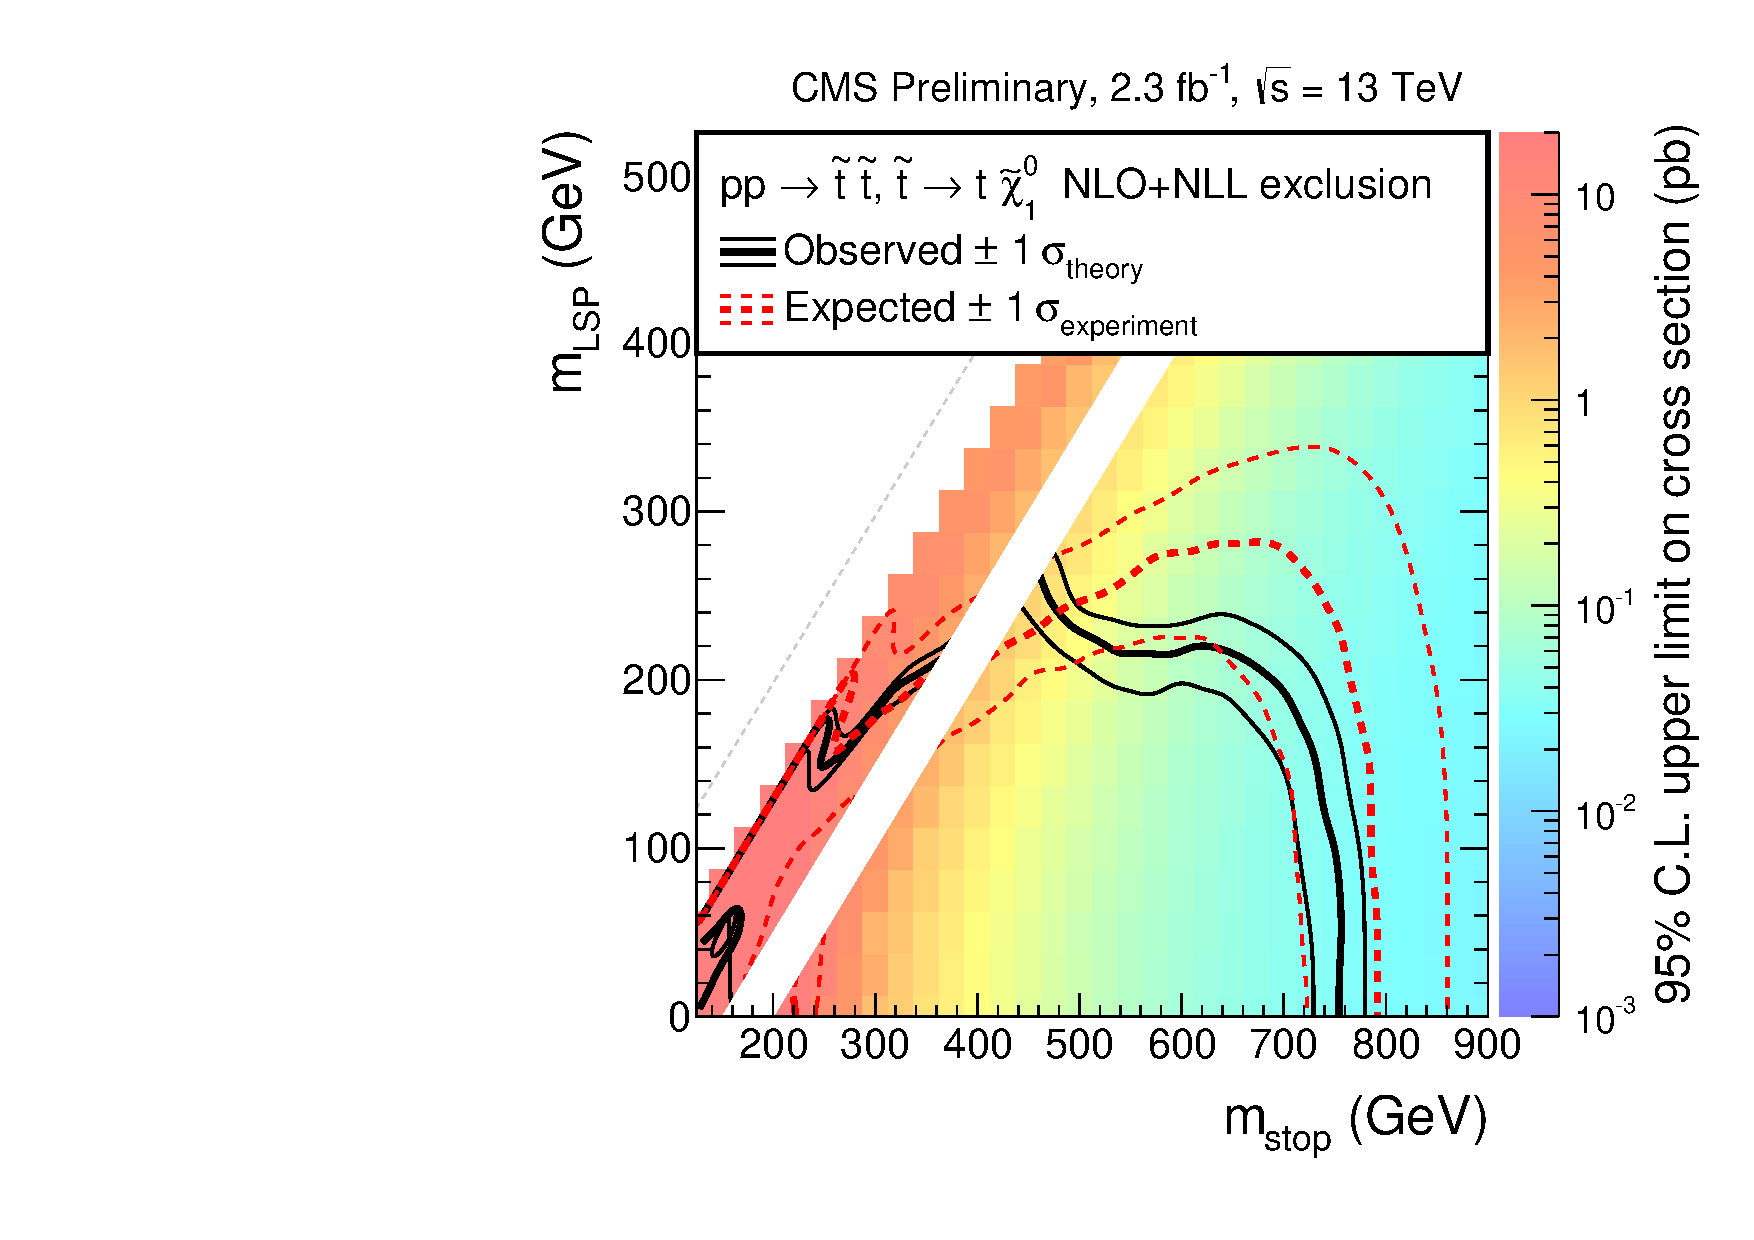
\includegraphics[angle=0,width=0.48\textwidth]{figures/Covered_BR_1p00_Stop_OnlyXSEC.pdf}
  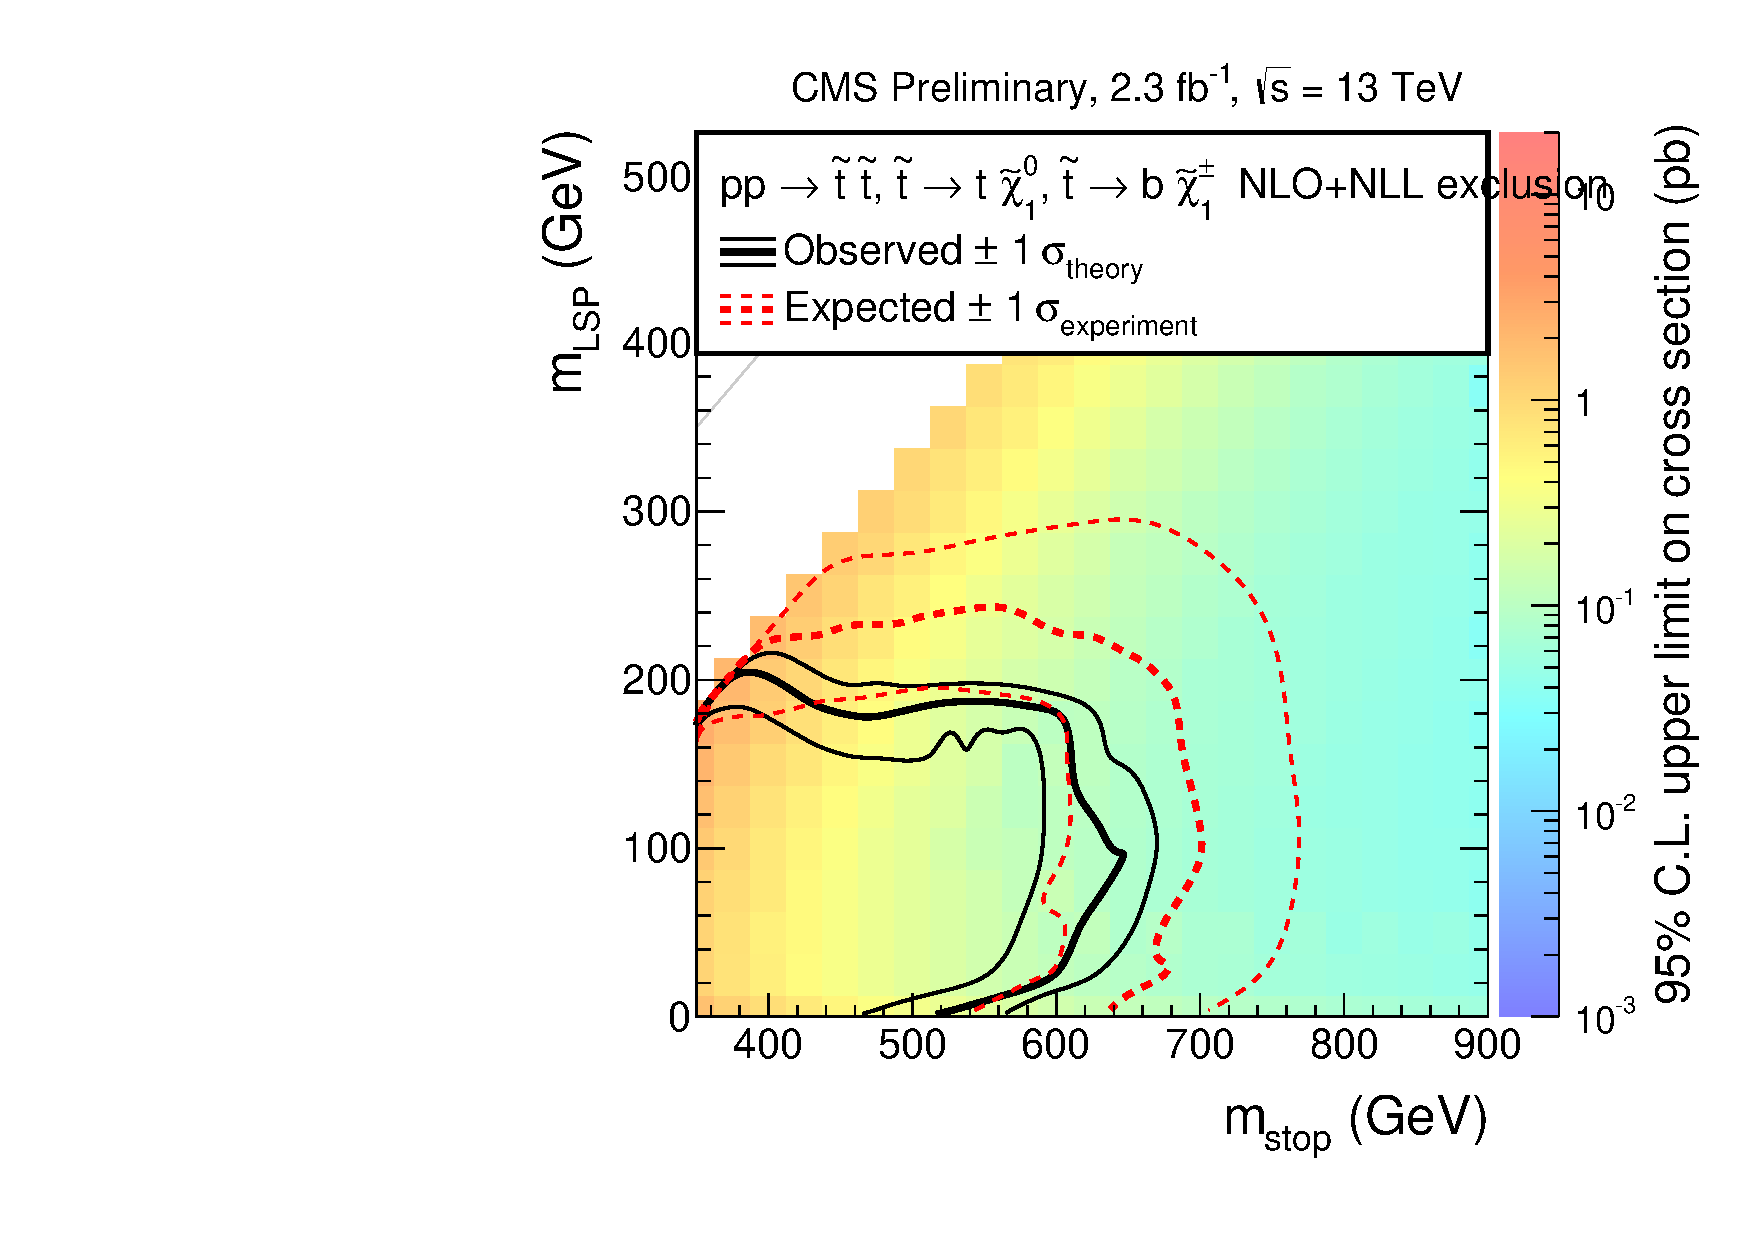
\includegraphics[angle=0,width=0.48\textwidth]{figures/BR_0p50_Stop_OnlyXSEC.pdf}
  \end{tabular}
  \caption{Expected limits and observed limits. The left shows the limits on the T2tt model, where the branching ratio for the top squark to decay to a top quark and neutralino is 100\%. The right plots shows the limits on the T2tb model, where the branching ratio for a top squark to decay to a top quark and neutralino is 50\%. }
    \label{fig:fulllimit_T2tt_T2tb}
  \end{center}
\end{figure}
%%%%%%%%%%%%%%%%%%%%%%%%%%%%%%%%%%%%%%%%%%%%%%%%%%
The observed exclusion curves are also shown for the cases in which the signal cross section is varied by changing the renormalization and factorization scales by a factor of 2 and using the PDF4LHC recommendation~\cite{Botje:2011sn} for the PDF uncertainty to illustrate the sensitivity of the exclusion to the signal cross section uncertainty.
%
The expected exclusion curves show the cases in which the background uncertainties are varied by one standard deviation.

In the T2tt model, shown in the left plot of Fig.~\ref{fig:fulllimit_T2tt_T2tb}, where both top squarks decay to top quarks and neutralinos, the median expected lower limit on the top squark mass reaches 790~\GeV, for small neutralino masses, and the observed limit excludes top squark masses below about 760~\GeV at 95\% confidence level.  
%
For large neutralino masses in the same model, the median expected lower mass limit on the neutralino reaches about 280~\GeV with an observed limit near 220~\GeV, for a top squark mass near 650~\GeV. 

In the T2tb model, displayed in the right plot f Fig.~\ref{fig:fulllimit_T2tt_T2tb}, which includes a light chargino (nearly degenerate with the neutralino) and allows the top squark to decay to a bottom quark and chargino with 50\% probability, the median expected lower limit reaches 700~\GeV, for a neutralino mass near 100~\GeV, and the observed limit excludes top squark masses below about 650~\GeV at 95\% confidence level. 
%
For larger neutralino masses, the median expected lower limit on the neutralino mass reaches about 240~\GeV with an observed limit near 200~\GeV. 









